\chapter{Kesetimbangan Kimia: Kuosien dan Tetapan}\label{ch:g12:equilibrium}

Sebotol air soda yang tertutup rapat tetap bergas selama berbulan-bulan;
setelah dibuka, air itu kehilangan gasnya dalam satu sore. Dalam kedua
kasus tidak ada yang salah. Di dalam botol tertutup, karbon dioksida
meninggalkan air dan kembali ke dalamnya dengan laju yang sama, dan
komposisinya tetap; bukalah tutupnya, dan gas yang keluar tidak lagi
kembali. Banyak reaksi berperilaku seperti ini: reaksi itu berhenti
sebelum ada \omterm{def:g7:chemical-reactions:reactant}{pereaksi} yang habis, pada keseimbangan antara dua reaksi
yang berlawanan. Bab ini menggambarkan keseimbangan itu dengan satu
bilangan.

\begin{recall}
Kemajuan $x$ sebuah reaksi, nilai maksimumnya $x_{\max}$, dan \omterm{def:g10:reaction-progress-table:limiting}{reaksi
tuntas} yang mencapainya (\cref{ch:g10:reaction-progress-table}). Laju
dan \omterm{def:g12:reaction-rates:kinetic-factor}{faktor kinetik} (\cref{ch:g12:reaction-rates}); \omterm{def:g12:catalysis:catalyst}{katalis} tidak
mengubah \omterm{def:g10:reaction-progress-table:system}{keadaan akhir} (\cref{ch:g12:catalysis}).
\end{recall}

\begin{omfigure}
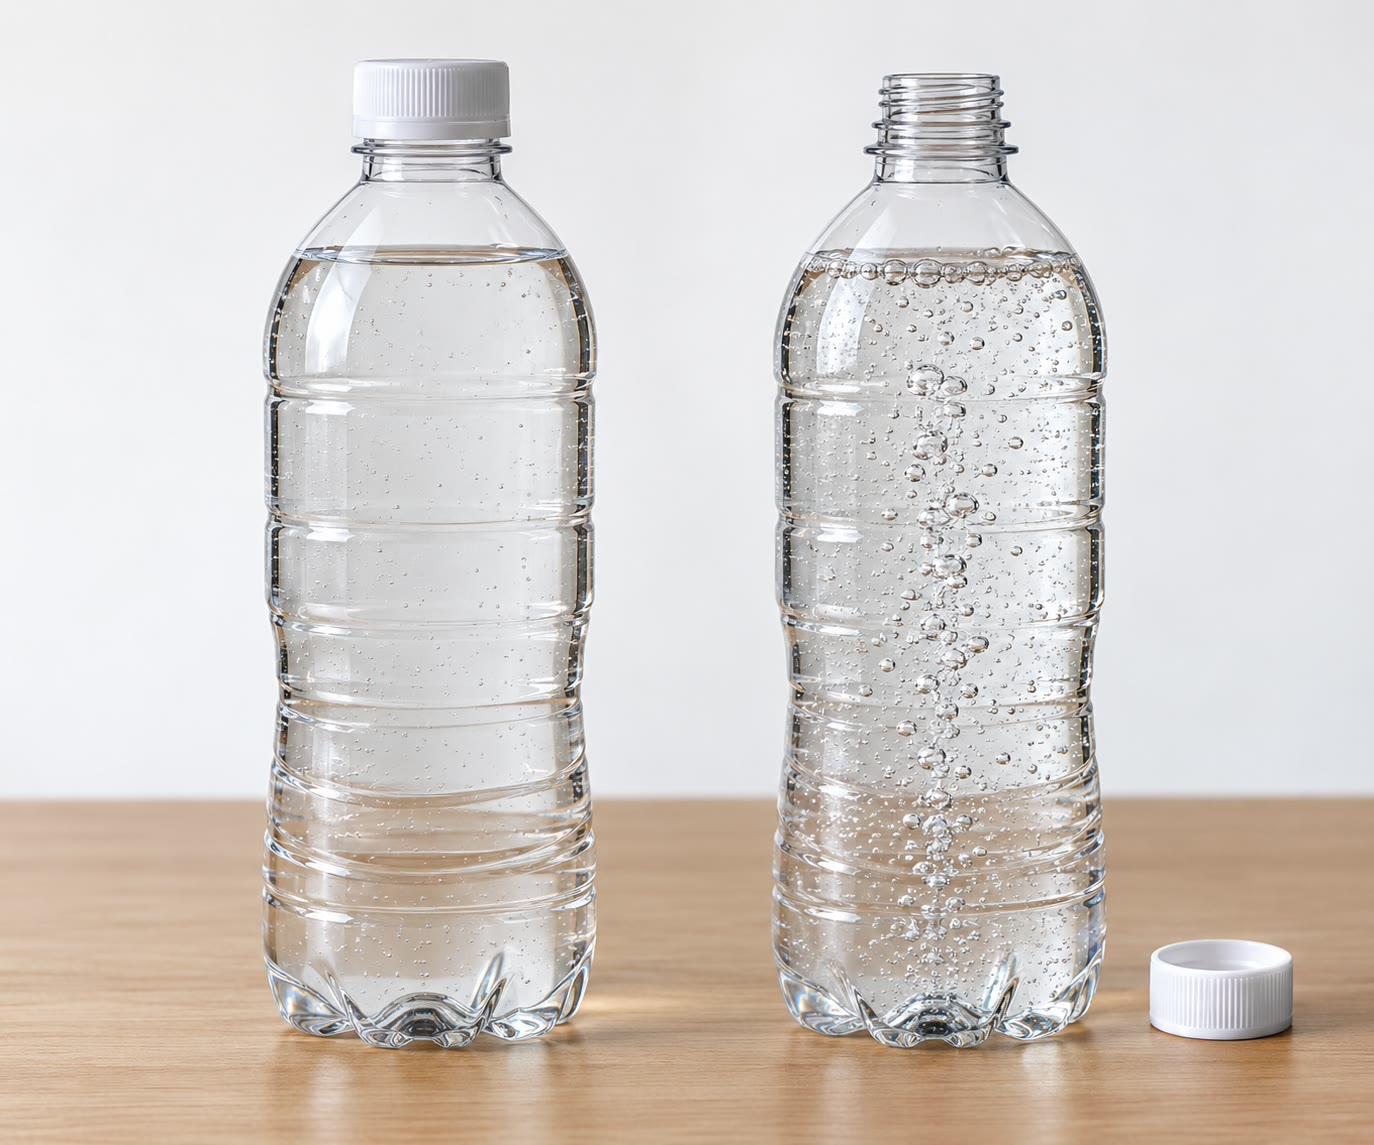
\includegraphics[width=0.45\linewidth,height=5cm,keepaspectratio]{images/book1/ai/g12-fizzy-bottles.jpg}

{\small Tertutup, air itu menyimpan gasnya; terbuka, gasnya keluar dan
tidak kembali.}
\end{omfigure}

\section{Reaksi yang tidak tuntas}

\begin{definition}[Reaksi tidak tuntas, rasio kemajuan akhir]\label{def:g12:equilibrium:non-total}
Sebuah reaksi disebut \emph{reaksi tidak tuntas}\index{reaksi tidak tuntas}
jika reaksi itu berhenti pada kemajuan akhir $x_f$ yang lebih kecil
daripada \omterm{def:g10:reaction-progress-table:limiting}{kemajuan maksimumnya} $x_{\max}$, dengan semua \omterm{def:g7:chemical-reactions:reactant}{pereaksinya} masih
ada. Yang disebut \emph{rasio kemajuan akhir}\index{rasio kemajuan akhir}
reaksi itu adalah
\[
  \tau = \frac{x_f}{x_{\max}}, \qquad 0 < \tau < 1
\]
($\tau = 1$ untuk \omterm{def:g10:reaction-progress-table:limiting}{reaksi tuntas}).
\end{definition}

\begin{example}[Ester yang berhenti di tengah jalan]\label{ex:g12:equilibrium:berthelot}
% ledger: ester:berthelot
Jika dipanaskan dengan \qty{1}{mol} etanol, \qty{1}{mol} asam etanoat
membentuk etil etanoat dan air,
\ce{CH3COOH + C2H5OH <=> CH3COOC2H5 + H2O}. Reaksinya berhenti ketika
sekitar dua pertiga asamnya telah bereaksi: $x_f = \qty{0.67}{mol}$
untuk $x_{\max} = \qty{1}{mol}$, jadi $\tau \approx 0.67$. Jika dimulai
dari \qty{1}{mol} \omterm{def:g11:functional-groups:carboxylic-acid}{ester} dan \qty{1}{mol} air, reaksi kebalikannya juga
berhenti, dengan sekitar sepertiga \omterm{def:g11:functional-groups:carboxylic-acid}{esternya} terhidrolisis: \omterm{def:g6:pure-substances-and-mixtures:mixture}{campuran}
akhirnya sama.
\end{example}

\begin{history}[Berthelot dan Péan de Saint-Gilles, 1862]
% ledger: ester:berthelot
Ahli kimia Marcellin Berthelot dan Léon Péan de Saint-Gilles memanaskan
\omterm{def:g6:pure-substances-and-mixtures:mixture}{campuran} asam etanoat dan etanol, serta \omterm{def:g6:pure-substances-and-mixtures:mixture}{campuran} etil etanoat dan air,
selama waktu yang lama, lalu menganalisisnya. Dari asam dan \omterm{def:g11:functional-groups:alcohol}{alkohol}
dalam jumlah yang sama, reaksinya selalu berhenti pada sekitar dua
pertiga; dari \omterm{def:g11:functional-groups:carboxylic-acid}{ester} dan air, pada sepertiga hidrolisis; dan mereka
memperhatikan bahwa jumlah \omterm{def:g11:functional-groups:carboxylic-acid}{ester} yang terbentuk pada setiap saat
bergantung pada hasil kali jumlah \omterm{def:g7:chemical-reactions:reactant}{pereaksinya}. Karya mereka termasuk
salah satu kajian kuantitatif pertama tentang kesetimbangan kimia.
\end{history}

\section{Keadaan kesetimbangan}

\begin{definition}[Keadaan kesetimbangan]\label{def:g12:equilibrium:equilibrium-state}
Sebuah sistem berada dalam \emph{keadaan
kesetimbangan}\index{keadaan kesetimbangan} jika komposisinya tidak lagi
berubah walaupun reaksi maju dan reaksi balik masih terus berlangsung,
dengan laju yang sama. Reaksi yang dapat mencapai keadaan semacam itu
ditulis dengan panah ganda $\rightleftharpoons$.
\end{definition}

\begin{omfigure}
\begin{tikzpicture}
\begin{axis}[width=0.8\linewidth, height=6cm, xmin=0, xmax=200, ymin=0,
    ymax=1.05, xlabel={$t$ (\si{h})}, ylabel={jumlah ester (\si{mol})},
    axis lines*=left, ymajorgrids, grid style={gray!20},
    tick label style={font=\small}, label style={font=\small},
    legend style={font=\small, at={(0.98,0.98)}, anchor=north east,
    draw=none, fill=white}, legend cell align=left]
  % ledger: ester:berthelot (K = 4; kinetics synthetic)
  \addplot[very thick, omDef] table[x=t, y=fromAcid] {figdata/out/grade-12-equilibrium.dat};
  \addplot[very thick, omProp] table[x=t, y=fromEster] {figdata/out/grade-12-equilibrium.dat};
  \addplot[dashed, black!60] coordinates {(0,0.6667) (200,0.6667)};
  \legend{dari 1 mol asam + 1 mol alkohol, dari 1 mol ester + 1 mol air}
  \node[font=\small, anchor=north east] at (axis cs:195,0.65) {kesetimbangan: $\tfrac{2}{3}$ mol};
\end{axis}
\end{tikzpicture}

{\small Esterifikasi (biru) dan hidrolisis \omterm{def:g11:functional-groups:carboxylic-acid}{ester} (jingga) mencapai
komposisi kesetimbangan yang sama, dari sisi yang berlawanan. (Skala
waktunya berasal dari model; nilai akhirnya adalah nilai terukur.)}
\end{omfigure}

\section{Kuosien reaksi}

\begin{notation}[Konsentrasi standar]\label{not:g12:equilibrium:c-standard}
$c^\circ = \qty{1}{mol/L}$ adalah konsentrasi standar. Membagi sebuah
konsentrasi dengan $c^\circ$ menghasilkan bilangan tanpa satuan yang
nilainya sama: $[\ce{A}]/c^\circ$.
\end{notation}

\begin{definition}[Kuosien reaksi]\label{def:g12:equilibrium:quotient}
Untuk reaksi dalam larutan $a\,\ce{A} + b\,\ce{B} \rightleftharpoons c\,\ce{C} + d\,\ce{D}$,
\emph{kuosien reaksi}\index{kuosien reaksi} pada suatu keadaan sistem
adalah
\[
  Q = \frac{\left([\ce{C}]/c^\circ\right)^c \left([\ce{D}]/c^\circ\right)^d}
           {\left([\ce{A}]/c^\circ\right)^a \left([\ce{B}]/c^\circ\right)^b} .
\]
Padatan, dan \omterm{def:g6:solutions-and-solubility:solute}{pelarutnya} (air dalam \omterm{def:g6:solutions-and-solubility:solute}{larutan berair}), tidak muncul dalam
$Q$.
\end{definition}


\begin{example}[Menuliskan kuosien]\label{ex:g12:equilibrium:quotients}
Untuk \ce{CH3COOH + H2O <=> CH3COO- + H3O+} dalam air (\omterm{def:g9:ions:ion}{ion} \ce{H3O+}
diperkenalkan pada bab berikutnya), air adalah \omterm{def:g6:solutions-and-solubility:solute}{pelarutnya}:
$Q = \dfrac{[\ce{CH3COO-}]\,[\ce{H3O+}]}{[\ce{CH3COOH}]\,c^\circ}$.
Untuk pelarutan sebuah padatan, \ce{AgCl(s) <=> Ag+ + Cl-}, padatannya
tidak dituliskan: $Q = [\ce{Ag+}][\ce{Cl-}]/(c^\circ)^2$. Untuk
esterifikasi, yang keempat spesiesnya berada dalam \omterm{def:g6:pure-substances-and-mixtures:mixture}{campuran} cair yang
sama bervolume $V$, volumenya saling meniadakan dan
$Q = \dfrac{n_{\text{ester}}\, n_{\text{air}}}{n_{\text{asam}}\, n_{\text{alkohol}}}$.
\end{example}

\section{Tetapan kesetimbangan}

\begin{definition}[Tetapan kesetimbangan]\label{def:g12:equilibrium:constant}
Nilai $Q_{eq}$ \omterm{def:g12:equilibrium:quotient}{kuosien reaksi} pada \omterm{def:g12:equilibrium:equilibrium-state}{keadaan kesetimbangan} disebut
\emph{tetapan kesetimbangan}\index{tetapan kesetimbangan} $K$ reaksi
itu. Tetapan ini tidak bersatuan.
\end{definition}

\begin{proposition}[$K$ hanya bergantung pada suhu]\label{prop:g12:equilibrium:constant}
Untuk suatu reaksi, $Q_{eq} = K$ pada setiap \omterm{def:g12:equilibrium:equilibrium-state}{keadaan kesetimbangan} pada
suhu tertentu, berapa pun jumlah awalnya.
\end{proposition}

\begin{proof}
Diterima tanpa bukti; hal ini diturunkan dalam buku Tahun Kedua
universitas. Hal ini diperiksa pada esterifikasi: kedua percobaan dalam
gambar, yang dimulai dari sisi berlawanan, memberikan $Q_{eq}$ yang
sama.
\end{proof}

\begin{example}[$K$ esterifikasi]\label{ex:g12:equilibrium:k-ester}
% ledger: ester:berthelot
Dari \qty{1}{mol} asam dan \qty{1}{mol} \omterm{def:g11:functional-groups:alcohol}{alkohol}, kesetimbangannya
mengandung $\frac{2}{3}$ \omterm{def:g10:the-mole:amount}{mol} \omterm{def:g11:functional-groups:carboxylic-acid}{ester} dan air serta $\frac{1}{3}$ \omterm{def:g10:the-mole:amount}{mol} asam
dan \omterm{def:g11:functional-groups:alcohol}{alkohol}:
\[
  K = \frac{(2/3)\times(2/3)}{(1/3)\times(1/3)} = 4 .
\]
\end{example}

\begin{method}[Keadaan akhir reaksi tidak tuntas]\label{met:g12:equilibrium:final}
\begin{enumerate}
  \item Isilah \omterm{def:g10:reaction-progress-table:extent}{tabel kemajuan} dengan kemajuan akhir $x_f$ yang belum
        diketahui.
  \item Tuliskan $Q_{eq}$ sebagai fungsi $x_f$ dan samakan dengan $K$.
  \item Selesaikan untuk $x_f$ (sering berupa persamaan kuadrat), dengan
        mempertahankan akar yang terletak antara 0 dan $x_{\max}$.
  \item Simpulkan jumlah akhirnya dan $\tau = x_f/x_{\max}$.
\end{enumerate}
\end{method}

\begin{example}[Alkohol berlebih]\label{ex:g12:equilibrium:excess}
Dari \qty{1}{mol} asam dan \qty{2}{mol} \omterm{def:g11:functional-groups:alcohol}{alkohol}:
$\dfrac{x^2}{(1-x)(2-x)} = 4$, yaitu $3x^2 - 12x + 8 = 0$, yang akarnya
antara 0 dan 1 adalah $x_f = \qty{0.845}{mol}$. Menggandakan \omterm{def:g11:functional-groups:alcohol}{alkohol}
menaikkan \omterm{def:g10:synthesis-yield:yield}{rendemen}, yang dihitung terhadap asam, dari \qty{67}{\percent}
menjadi \qty{85}{\percent}.
\end{example}

\section{Meramalkan dan menggeser arah perubahan}

\begin{proposition}[Arah perubahan]\label{prop:g12:equilibrium:direction}
Jika $Q < K$, sistem berubah ke arah maju (produknya bertambah) sampai
$Q = K$; jika $Q > K$, sistem berubah ke arah balik; jika $Q = K$,
sistem berada dalam kesetimbangan dan tidak berubah.
\end{proposition}

\begin{proof}
Diterima tanpa bukti: $Q$ bertambah ketika reaksi maju berlangsung
(produk di pembilang bertambah, \omterm{def:g7:chemical-reactions:reactant}{pereaksi} di penyebut berkurang), dan
sistem bergerak menuju keadaan dengan $Q = K$.
\end{proof}

\begin{omfigure}
\begin{tikzpicture}[font=\small]
  \draw[->, thick] (0,0) -- (10,0) node[right] {$Q$};
  \draw[thick] (0,-0.12) -- (0,0.12) node[above] {0};
  \draw[very thick, omThm] (5,-0.25) -- (5,0.25) node[above] {$K$};
  \draw[->, very thick, omDef] (1.2,0.55) -- (4.4,0.55);
  \node[omDef, align=center] at (2.8,1.15) {$Q < K$: maju};
  \draw[->, very thick, omProp] (8.8,0.55) -- (5.6,0.55);
  \node[omProp, align=center] at (7.2,1.15) {$Q > K$: balik};
  \node[align=center] at (5,-0.75) {$Q = K$: kesetimbangan};
\end{tikzpicture}

{\small Kuosien selalu bergerak menuju tetapan.}
\end{omfigure}

\begin{remark}[Menggeser kesetimbangan]\label{rem:g12:equilibrium:shift}
Untuk memperoleh lebih banyak produk dari reaksi yang tidak tuntas,
kita dapat menambahkan salah satu \omterm{def:g7:chemical-reactions:reactant}{pereaksi} secara berlebih (yang lebih
murah), atau mengambil sebuah produk selagi terbentuk: masing-masing
membuat $Q < K$ lagi, dan sistem bergerak maju. Mengambil air hasil
esterifikasi (dengan zat pengering, atau dengan menyulingnya) dapat
mendorong reaksi hampir sampai tuntas. Botol air soda yang terbuka
melakukan hal yang sama dengan karbon dioksida yang keluar.
\end{remark}

\begin{omfigure}
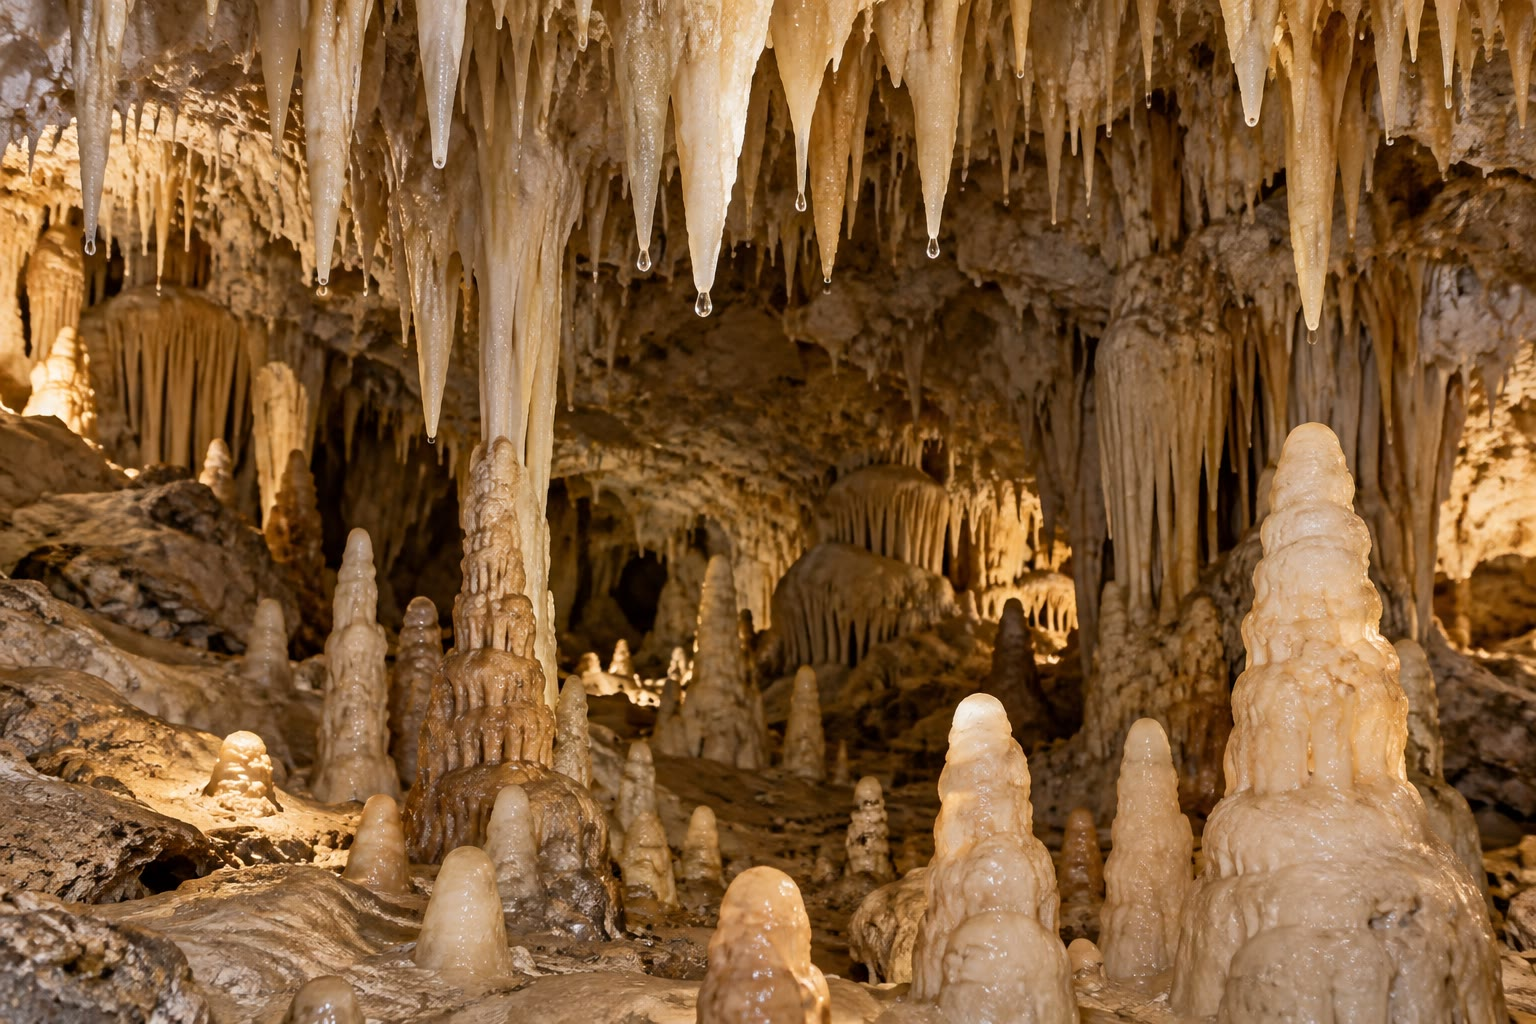
\includegraphics[width=0.45\linewidth]{images/book1/ai/g12-cave-stalactites.jpg}

{\small Stalaktit tumbuh di tempat air yang menetes di dalam gua
kehilangan karbon dioksida ke \omterm{def:g4:air-a-mixture-of-gases:air}{udara}: sebuah kesetimbangan batu kapur
terlarut tergeser, dan kalsium karbonat mengendap.}
\end{omfigure}

\section{Latihan}

\begin{exercise}[$\star$]\label{exo:g12:equilibrium:1}
Tuliskan \omterm{def:g12:equilibrium:quotient}{kuosien reaksi} untuk: (a) \ce{N2 + 3H2 <=> 2NH3} (gas, pakailah
konsentrasi); (b) \ce{CH3COOH + H2O <=> CH3COO- + H3O+} dalam air;
(c) \ce{CaCO3(s) <=> Ca^{2+} + CO3^{2-}}; (d) \ce{Fe^{3+} + SCN- <=>
FeSCN^{2+}}.
\end{exercise}

\begin{exercise}[$\star$]\label{exo:g12:equilibrium:2}
Sebuah reaksi memiliki $x_{\max} = \qty{0.050}{mol}$ dan mencapai
$x_f = \qty{0.020}{mol}$. Hitung $\tau$. Apakah reaksinya tuntas?
\end{exercise}

\begin{exercise}[$\star$]\label{exo:g12:equilibrium:3}
Untuk reaksi dengan $K = 10$, ke arah mana sebuah \omterm{def:g6:pure-substances-and-mixtures:mixture}{campuran} berubah jika
$Q = 2$? Jika $Q = 50$? Jika $Q = 10$?
\end{exercise}

\begin{exercise}[$\star$]\label{exo:g12:equilibrium:4}
Jelaskan mengapa kesetimbangan disebut ``dinamis''.
\end{exercise}

\begin{exercise}[$\star$]\label{exo:g12:equilibrium:5}
Apakah \omterm{def:g12:catalysis:catalyst}{katalis} mengubah $K$? Mengubah waktu yang diperlukan untuk
mencapai kesetimbangan? Jelaskan.
\end{exercise}

\begin{exercise}[$\star\star$]\label{exo:g12:equilibrium:6}
Sebanyak \qty{2.0}{mol} asam etanoat dan \qty{2.0}{mol} etanol
\omterm{def:g2:mixing-and-dissolving:mix}{dicampur} ($K = 4$). Hitung jumlah akhir keempat spesies.
\end{exercise}

\begin{exercise}[$\star\star$]\label{exo:g12:equilibrium:7}
Sebuah \omterm{def:g6:pure-substances-and-mixtures:mixture}{campuran} mengandung masing-masing \qty{0.5}{mol} asam etanoat,
etanol, etil etanoat, dan air. Hitung $Q$. Ke arah mana \omterm{def:g6:pure-substances-and-mixtures:mixture}{campuran} itu
berubah?
\end{exercise}

\begin{exercise}[$\star\star$]\label{exo:g12:equilibrium:8}
Dengan gambar kedua percobaan, bacalah jumlah \omterm{def:g11:functional-groups:carboxylic-acid}{ester} setelah
\qty{20}{h} pada setiap percobaan. Kapan sistem dapat dianggap berada
dalam kesetimbangan?
\end{exercise}

\begin{exercise}[$\star\star$]\label{exo:g12:equilibrium:9}
Dimulai dari \qty{1}{mol} \omterm{def:g11:functional-groups:carboxylic-acid}{ester} dan \qty{1}{mol} air ($K = 4$ untuk
esterifikasi, jadi $1/4$ untuk hidrolisis), hitung jumlah akhirnya
dengan metode dalam bab ini, lalu bandingkan dengan percobaan
esterifikasi.
\end{exercise}

\begin{exercise}[$\star\star$]\label{exo:g12:equilibrium:10}
Mengapa padatan tidak muncul dalam kuosien
\ce{AgCl(s) <=> Ag+ + Cl-}? Apakah penambahan padatan menggeser
kesetimbangannya?
\end{exercise}

\begin{exercise}[$\star\star$]\label{exo:g12:equilibrium:11}
Di dalam botol air soda yang tertutup, karbon dioksida meninggalkan dan
memasuki air dengan laju yang sama. Tuliskan kesetimbangan
\ce{CO2(aq) <=> CO2(g)}, lalu jelaskan, dengan $Q$ dan $K$, mengapa air
itu kehilangan gasnya ketika botolnya dibuka.
\end{exercise}

\begin{exercise}[$\star\star\star$]\label{exo:g12:equilibrium:12}
Esterifikasi \qty{1}{mol} asam dan \qty{1}{mol} \omterm{def:g11:functional-groups:alcohol}{alkohol} mencapai
kesetimbangan. Setengah dari air yang ada lalu diambil. Hitung $Q$ yang
baru, tentukan ke arah mana sistem berubah, dan temukan jumlah akhir
\omterm{def:g11:functional-groups:carboxylic-acid}{ester} yang baru.
\end{exercise}

\begin{exercise}[$\star\star\star$]\label{exo:g12:equilibrium:13}
Tunjukkan bahwa tetapan reaksi kebalikannya adalah $1/K$. Berapa tetapan
hidrolisis etil etanoat?
\end{exercise}

\begin{exercise}[$\star\star\star$]\label{exo:g12:equilibrium:14}
Seorang ahli kimia \omterm{def:g2:mixing-and-dissolving:mix}{mencampur} \qty{1}{mol} asam, \qty{1}{mol} \omterm{def:g11:functional-groups:alcohol}{alkohol},
\qty{2}{mol} \omterm{def:g11:functional-groups:carboxylic-acid}{ester}, dan \qty{0.5}{mol} air. Akankah terjadi sesuatu?
Jelaskan.
\end{exercise}

\begin{exercise}[$\star\star\star$]\label{exo:g12:equilibrium:15}
Berapa \omterm{def:g11:functional-groups:alcohol}{alkohol} berlebih (jumlah per \omterm{def:g10:the-mole:amount}{mol} asam) yang diperlukan untuk
mengesterkan \qty{95}{\percent} asamnya? Selesaikan
$\dfrac{0.95^2}{0.05(n - 0.95)} =
4$.
\end{exercise}

\section{Soal: Ester Berthelot}

\begin{problem}[{Soal akhir pekan --- berapa ester yang terbentuk jika
alkoholnya dibuat tiga kali berlebih?}]
\label{pb:g12:equilibrium:1}
% ledger: ester:berthelot, aw:C, aw:H, aw:O
Etil etanoat, sebuah \omterm{def:g6:solutions-and-solubility:solute}{pelarut} dan perisa, dibuat dari asam etanoat dan
etanol. Pada tahun 1862, Berthelot dan Péan de Saint-Gilles menemukan
bahwa dari asam dan \omterm{def:g11:functional-groups:alcohol}{alkohol} dalam jumlah yang sama, reaksinya berhenti
ketika sekitar dua pertiga asamnya telah bereaksi.

\medskip
\noindent\textbf{Bagian I --- Reaksinya.}
\begin{enumerate}
  \item Tuliskan persamaan esterifikasinya, dengan \omterm{def:g11:organic-skeletons:formulas}{rumus struktur
        ringkas}.
  \item Mengapa persamaan itu ditulis dengan panah ganda?
  \item Tuliskan \omterm{def:g12:equilibrium:quotient}{kuosien reaksinya} dalam \omterm{def:g10:the-mole:amount}{jumlah zat}.
  \item Dari \qty{1}{mol} asam dan \qty{1}{mol} \omterm{def:g11:functional-groups:alcohol}{alkohol}, berapa
        $x_{\max}$? Berapa $x_f$, menurut hasil Berthelot?
  \item Hitung $\tau$.
\end{enumerate}

\medskip
\noindent\textbf{Bagian II --- Tetapannya.}
\begin{enumerate}[resume]
  \item Berikan jumlah akhir keempat spesies itu.
  \item Hitung $K$.
  \item Dimulai dari \qty{1}{mol} \omterm{def:g11:functional-groups:carboxylic-acid}{ester} dan \qty{1}{mol} air, Berthelot
        mendapati sepertiganya terhidrolisis. Tunjukkan bahwa hasil ini
        sesuai dengan $K$ yang sama.
  \item Mengapa $K$ harus sama pada kedua kasus?
\end{enumerate}

\medskip
\noindent\textbf{Bagian III --- \omterm{def:g11:functional-groups:alcohol}{Alkohol} tiga kali berlebih.}
\begin{enumerate}[resume]
  \item Dari \qty{1}{mol} asam dan \qty{3}{mol} \omterm{def:g11:functional-groups:alcohol}{alkohol}, isilah \omterm{def:g10:reaction-progress-table:extent}{tabel
        kemajuannya}.
  \item Tuliskan persamaan $Q_{eq} = K$ lalu tunjukkan bahwa persamaan
        itu menjadi $3x^2 - 16x + 12 = 0$.
  \item Selesaikan persamaan itu, dan pertahankan akar yang bermakna.
  \item Berapa bagian asam yang teresterkan?
  \item Hitung massa \omterm{def:g11:functional-groups:carboxylic-acid}{ester} yang diperoleh.
\end{enumerate}

\medskip
\noindent\textbf{Bagian IV --- Mengambil air.}
\begin{enumerate}[resume]
  \item Dari kesetimbangan ekuimolar, air diambil selagi terbentuk.
        Jelaskan dengan $Q$ mengapa reaksinya terus berlangsung.
  \item Jika seluruh air dapat diambil, berapa \omterm{def:g10:synthesis-yield:yield}{rendemennya}?
  \item Mengapa \omterm{def:g11:functional-groups:alcohol}{alkohol}, bukan asam, yang biasanya dibuat berlebih?
        (Pikirkan harganya dan pemisahan produknya.)
  \item Apakah pemanasan \omterm{def:g6:pure-substances-and-mixtures:mixture}{campuran} mengubah \omterm{def:g10:reaction-progress-table:system}{keadaan akhirnya}, atau hanya
        waktu untuk mencapainya? (Esterifikasi hampir tidak melepaskan
        panas.)
  \item Nyatakan jawaban akhirnya: berapa bagian asam yang teresterkan
        dengan \omterm{def:g11:functional-groups:alcohol}{alkohol} tiga kali berlebih?
\end{enumerate}
\end{problem}
